% ===========================================================================
%  TikuOS — Memory Management: Pool Allocator
%  Beamer Presentation
% ===========================================================================
\documentclass[aspectratio=169, 10pt]{beamer}

% ---- Theme ----------------------------------------------------------------
\usetheme{Madrid}
\usecolortheme{whale}
\setbeamertemplate{navigation symbols}{}
\setbeamertemplate{footline}{%
  \leavevmode\hbox{%
    \begin{beamercolorbox}[wd=.33\paperwidth,ht=2.5ex,dp=1ex,center]{author in head/foot}%
      \usebeamerfont{author in head/foot}\insertshortauthor
    \end{beamercolorbox}%
    \begin{beamercolorbox}[wd=.34\paperwidth,ht=2.5ex,dp=1ex,center]{title in head/foot}%
      \usebeamerfont{title in head/foot}\insertshorttitle
    \end{beamercolorbox}%
    \begin{beamercolorbox}[wd=.33\paperwidth,ht=2.5ex,dp=1ex,right]{date in head/foot}%
      \usebeamerfont{date in head/foot}\insertshortdate{}\hspace*{2em}%
      \insertframenumber{}/\inserttotalframenumber\hspace*{2ex}
    \end{beamercolorbox}}%
  \vskip0pt%
}

% ---- Packages -------------------------------------------------------------
\usepackage{listings}
\usepackage{graphicx}
\usepackage{hyperref}
\usepackage{booktabs}
\usepackage{multirow}
\usepackage{tikz}
\usetikzlibrary{arrows.meta, positioning, shapes.geometric, calc, decorations.pathreplacing}

% ---- Code listing style ---------------------------------------------------
\lstset{
  basicstyle=\ttfamily\scriptsize,
  keywordstyle=\color{blue}\bfseries,
  commentstyle=\color{gray},
  stringstyle=\color{red!70!black},
  showstringspaces=false,
  breaklines=true,
  frame=single,
  rulecolor=\color{black!30},
  backgroundcolor=\color{blue!3},
  tabsize=4,
}
\lstdefinestyle{cstyle}{
  language=C,
  morekeywords={uint8_t,uint16_t,uint32_t,tiku_pool_t,tiku_mem_stats_t,
                tiku_mem_err_t,tiku_mem_arch_size_t,TIKU_MEM_OK,
                TIKU_MEM_ERR_INVALID,TIKU_MEM_ERR_NOMEM,NULL},
}
\lstdefinestyle{bashstyle}{
  language=bash,
  morekeywords={sudo,apt,make,gcc},
}

% ---- Metadata -------------------------------------------------------------
\title[TikuOS Pool]{TikuOS Pool Allocator}
\subtitle{Simple. Ubiquitous. Intelligence, Everywhere.}
\author[Ambuj Varshney]{Ambuj Varshney \\ \texttt{ambuj@tiku-os.org}}
\date{\today}

% ===========================================================================
\begin{document}

% ---------------------------------------------------------------------------
\begin{frame}
\titlepage
\end{frame}

% ---------------------------------------------------------------------------
\begin{frame}{Outline}
\tableofcontents
\end{frame}

% ===========================================================================
\section{Why a Pool Allocator?}
% ===========================================================================

\begin{frame}{Arena vs.\ Pool: Complementary Strategies}
\begin{columns}[T]
\begin{column}{0.48\textwidth}
\textbf{Arena (bump-pointer):}
\begin{itemize}
  \item O(1) alloc, O(1) bulk free
  \item No individual free
  \item Ideal for shared-lifetime buffers
  \item Zero fragmentation
\end{itemize}

\vspace{0.5em}
\begin{block}{Arena Limitation}
Cannot free individual objects. All allocations must be
discarded together via \texttt{reset()}.
\end{block}
\end{column}

\begin{column}{0.48\textwidth}
\textbf{Pool (fixed-size block):}
\begin{itemize}
  \item O(1) alloc, O(1) individual free
  \item Embedded freelist --- zero metadata
  \item Ideal for alloc/free of equal-sized objects
  \item Zero fragmentation
\end{itemize}

\vspace{0.5em}
\begin{block}{Pool Use Cases}
Packet buffers, message slots, sensor sample records,
timer descriptors --- any pattern needing individual
alloc/free of fixed-size objects.
\end{block}
\end{column}
\end{columns}
\end{frame}

% ===========================================================================
\section{Architecture \& Data Structures}
% ===========================================================================

\begin{frame}[fragile]{Pool Control Block}
\begin{columns}[T]
\begin{column}{0.50\textwidth}
\begin{lstlisting}[style=cstyle, title={kernel/memory/tiku\_mem.h}]
typedef struct {
    uint8_t *buf;
    tiku_mem_arch_size_t block_size;
    tiku_mem_arch_size_t block_count;
    void    *free_head;
    tiku_mem_arch_size_t used_count;
    tiku_mem_arch_size_t peak_count;
    uint8_t  id;
    uint8_t  active;
} tiku_pool_t;
\end{lstlisting}
\end{column}

\begin{column}{0.46\textwidth}
\begin{tabular}{@{}lp{4.5cm}@{}}
\toprule
\textbf{Field} & \textbf{Purpose} \\
\midrule
\texttt{buf}         & Caller-provided backing buffer \\
\texttt{block\_size}  & Aligned size of each block \\
\texttt{block\_count} & Total number of blocks \\
\texttt{free\_head}   & Head of embedded freelist \\
\texttt{used\_count}  & Currently allocated blocks \\
\texttt{peak\_count}  & Lifetime high-water mark \\
\texttt{id}          & Debug identifier (0--255) \\
\texttt{active}      & Non-zero if initialized \\
\bottomrule
\end{tabular}
\end{column}
\end{columns}

\vspace{0.5em}
\begin{block}{Key Design}
Like the arena, the pool \textbf{does not own} the buffer --- the caller
provides a statically allocated array. No dynamic allocation anywhere.
\end{block}
\end{frame}

% ---------------------------------------------------------------------------
\begin{frame}[fragile]{The Embedded Freelist}
\begin{center}
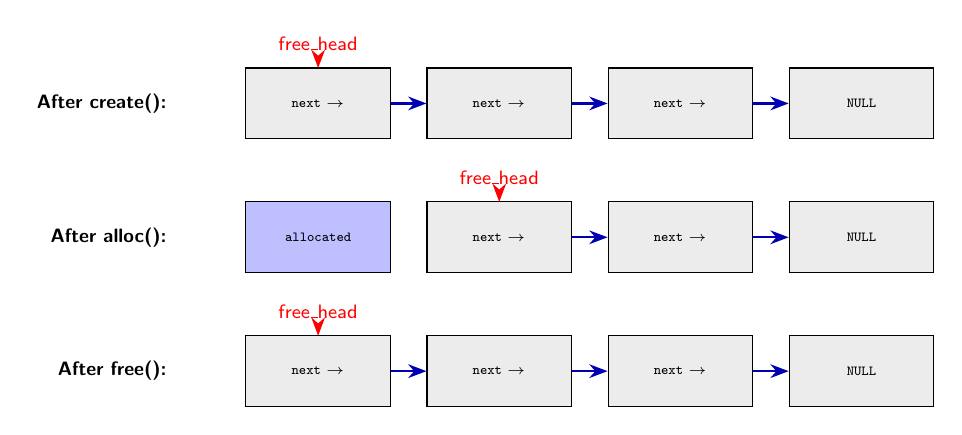
\begin{tikzpicture}[
    block/.style={draw, minimum width=1.8cm, minimum height=0.9cm,
                  font=\tiny\ttfamily, text width=1.6cm, align=center},
    ptr/.style={->, >=Stealth, thick, blue!70!black},
    label/.style={font=\scriptsize\sffamily},
    >=Stealth
  ]

  % --- After create: freelist chains all blocks ---
  \node[label, anchor=east] at (-0.3, 0) {\textbf{After create():}};
  \node[block, fill=gray!15] (b0) at (1.5, 0) {next $\rightarrow$};
  \node[block, fill=gray!15] (b1) at (3.8, 0) {next $\rightarrow$};
  \node[block, fill=gray!15] (b2) at (6.1, 0) {next $\rightarrow$};
  \node[block, fill=gray!15] (b3) at (8.4, 0) {NULL};
  \draw[ptr] (b0.east) -- (b1.west);
  \draw[ptr] (b1.east) -- (b2.west);
  \draw[ptr] (b2.east) -- (b3.west);
  \node[label, red, anchor=south] at (1.5, 0.55) {free\_head};
  \draw[thick, red, ->] (1.5, 0.55) -- (1.5, 0.45);

  % --- After alloc(): pop head ---
  \node[label, anchor=east] at (-0.3, -1.7) {\textbf{After alloc():}};
  \node[block, fill=blue!25] (c0) at (1.5, -1.7) {allocated};
  \node[block, fill=gray!15] (c1) at (3.8, -1.7) {next $\rightarrow$};
  \node[block, fill=gray!15] (c2) at (6.1, -1.7) {next $\rightarrow$};
  \node[block, fill=gray!15] (c3) at (8.4, -1.7) {NULL};
  \draw[ptr] (c1.east) -- (c2.west);
  \draw[ptr] (c2.east) -- (c3.west);
  \node[label, red, anchor=south] at (3.8, -1.15) {free\_head};
  \draw[thick, red, ->] (3.8, -1.15) -- (3.8, -1.25);

  % --- After free(): push onto head ---
  \node[label, anchor=east] at (-0.3, -3.4) {\textbf{After free():}};
  \node[block, fill=gray!15] (d0) at (1.5, -3.4) {next $\rightarrow$};
  \node[block, fill=gray!15] (d1) at (3.8, -3.4) {next $\rightarrow$};
  \node[block, fill=gray!15] (d2) at (6.1, -3.4) {next $\rightarrow$};
  \node[block, fill=gray!15] (d3) at (8.4, -3.4) {NULL};
  \draw[ptr] (d0.east) -- (d1.west);
  \draw[ptr] (d1.east) -- (d2.west);
  \draw[ptr] (d2.east) -- (d3.west);
  \node[label, red, anchor=south] at (1.5, -2.85) {free\_head};
  \draw[thick, red, ->] (1.5, -2.85) -- (1.5, -2.95);

\end{tikzpicture}
\end{center}

\vspace{0.3em}
\begin{alertblock}{Zero Metadata Overhead}
Each free block stores the next-pointer \textbf{inside its own memory}
(first \texttt{sizeof(void *)} bytes). When allocated, those bytes are
returned to the caller. No separate metadata structure needed.
\end{alertblock}
\end{frame}

% ---------------------------------------------------------------------------
\begin{frame}[fragile]{Building the Freelist}
\begin{lstlisting}[style=cstyle, title={kernel/memory/tiku\_pool.c (private helper)}]
static void build_freelist(tiku_pool_t *pool)
{
    tiku_mem_arch_size_t i;
    uint8_t *block;
    void **next_ptr;

    for (i = 0; i < pool->block_count - 1U; i++) {
        block    = pool->buf + (i * pool->block_size);
        next_ptr = (void **)(void *)block;
        *next_ptr = block + pool->block_size;
    }

    /* Last block terminates the list */
    block    = pool->buf + ((pool->block_count - 1U) * pool->block_size);
    next_ptr = (void **)(void *)block;
    *next_ptr = NULL;

    pool->free_head = pool->buf;
}
\end{lstlisting}

\begin{block}{Why \texttt{uint8\_t *} Pointer Arithmetic}
Struct padding and pointer size vary across platforms. By casting
to \texttt{uint8\_t *} and indexing by \texttt{i * block\_size}, we get exact
byte-offset arithmetic that works on 16-bit MSP430 and 64-bit hosts.
\end{block}
\end{frame}

% ===========================================================================
\section{API Reference}
% ===========================================================================

\begin{frame}[fragile]{tiku\_pool\_create()}
\begin{lstlisting}[style=cstyle]
tiku_mem_err_t tiku_pool_create(tiku_pool_t *pool, uint8_t *buf,
                                 tiku_mem_arch_size_t block_size,
                                 tiku_mem_arch_size_t block_count,
                                 uint8_t id);
\end{lstlisting}

\begin{itemize}
  \item Divides the buffer into \texttt{block\_count} blocks of \texttt{block\_size} bytes
  \item Rounds \texttt{block\_size} up to \texttt{TIKU\_MEM\_ARCH\_ALIGNMENT}
  \item Clamps to minimum of \texttt{sizeof(void *)} --- room for the freelist pointer
  \item Chains all blocks into the embedded freelist
  \item Returns \texttt{TIKU\_MEM\_ERR\_INVALID} if \texttt{pool} or \texttt{buf} is NULL, or \texttt{block\_count} is 0
\end{itemize}

\vspace{0.3em}
\textbf{Usage:}
\begin{lstlisting}[style=cstyle]
static uint8_t pkt_buf[8 * 64];  /* 8 blocks of 64 bytes */
static tiku_pool_t pkt_pool;

tiku_pool_create(&pkt_pool, pkt_buf, 64, 8, 1);
\end{lstlisting}
\end{frame}

% ---------------------------------------------------------------------------
\begin{frame}[fragile]{tiku\_pool\_alloc() \& tiku\_pool\_free()}
\begin{columns}[T]
\begin{column}{0.48\textwidth}
\begin{lstlisting}[style=cstyle, title={Alloc --- O(1), pop freelist}]
void *tiku_pool_alloc(
    tiku_pool_t *pool)
{
    void *block;
    void **next_ptr;

    if (pool == NULL || !pool->active
        || pool->free_head == NULL)
        return NULL;

    /* Pop head */
    block = pool->free_head;
    next_ptr = (void **)(void *)block;
    pool->free_head = *next_ptr;

    pool->used_count++;
    if (pool->used_count >
        pool->peak_count)
        pool->peak_count =
            pool->used_count;

    return block;
}
\end{lstlisting}
\end{column}

\begin{column}{0.48\textwidth}
\begin{lstlisting}[style=cstyle, title={Free --- O(1), push freelist}]
tiku_mem_err_t tiku_pool_free(
    tiku_pool_t *pool, void *ptr)
{
    uint8_t *block = (uint8_t *)ptr;
    tiku_mem_arch_size_t offset;
    void **next_ptr;

    /* Validate: in range? */
    if (block < pool->buf ||
        block >= pool->buf +
        (pool->block_count *
         pool->block_size))
        return TIKU_MEM_ERR_INVALID;

    /* Validate: aligned? */
    offset = (tiku_mem_arch_size_t)
        (block - pool->buf);
    if (offset % pool->block_size != 0)
        return TIKU_MEM_ERR_INVALID;

    /* Push onto head */
    next_ptr = (void **)(void *)block;
    *next_ptr = pool->free_head;
    pool->free_head = block;
    pool->used_count--;
    return TIKU_MEM_OK;
}
\end{lstlisting}
\end{column}
\end{columns}
\end{frame}

% ---------------------------------------------------------------------------
\begin{frame}[fragile]{Free Pointer Validation}
\begin{columns}[T]
\begin{column}{0.55\textwidth}
\texttt{tiku\_pool\_free()} performs two safety checks before
accepting a pointer:

\vspace{0.5em}
\begin{enumerate}
  \item \textbf{Range check:} \texttt{ptr} must fall within
        \texttt{[buf, buf + block\_count * block\_size)}
  \item \textbf{Alignment check:} \texttt{(ptr - buf) \% block\_size == 0}
\end{enumerate}

\vspace{0.5em}
This catches common embedded bugs:
\begin{itemize}
  \item Freeing a pointer from a different allocator
  \item Freeing a stack or heap pointer
  \item Freeing at the wrong offset within a block
\end{itemize}
\end{column}

\begin{column}{0.41\textwidth}
\begin{alertblock}{No MMU on MCUs}
On a microcontroller with no MMU, a stray free corrupts the
freelist silently, causing future allocs to return wild pointers.
The validation catches this at the point of error.
\end{alertblock}

\vspace{0.5em}
\begin{block}{Cost}
Two comparisons + one modulo operation.
Negligible compared to the consequences of silent
freelist corruption.
\end{block}
\end{column}
\end{columns}
\end{frame}

% ---------------------------------------------------------------------------
\begin{frame}[fragile]{Alignment \& Minimum Block Size}
\begin{lstlisting}[style=cstyle, title={kernel/memory/tiku\_pool.c (private helpers)}]
static tiku_mem_arch_size_t align_up(tiku_mem_arch_size_t size)
{
    const tiku_mem_arch_size_t mask = TIKU_MEM_ARCH_ALIGNMENT - 1U;
    return (size + mask) & ~mask;
}

static tiku_mem_arch_size_t min_block_size(void)
{
    tiku_mem_arch_size_t ptr_size = (tiku_mem_arch_size_t)sizeof(void *);
    if (TIKU_MEM_ARCH_ALIGNMENT > ptr_size)
        ptr_size = TIKU_MEM_ARCH_ALIGNMENT;
    return align_up(ptr_size);
}
\end{lstlisting}

\vspace{0.3em}
\begin{columns}[T]
\begin{column}{0.48\textwidth}
\begin{block}{Why \texttt{min\_block\_size()}?}
Each free block must hold at least one pointer for the embedded
freelist. On MSP430, \texttt{sizeof(void *) = 2}. On a 64-bit host,
it is 8. The minimum is \texttt{max(sizeof(void *), alignment)},
then rounded up.
\end{block}
\end{column}
\begin{column}{0.48\textwidth}
\begin{table}
\centering
\small
\begin{tabular}{@{}lcc@{}}
\toprule
\textbf{Platform} & \textbf{Alignment} & \textbf{Min Block} \\
\midrule
MSP430 (16-bit) & 2 & 2 \\
ARM Cortex-M    & 4 & 4 \\
x86-64 host     & 4 & 8 \\
\bottomrule
\end{tabular}
\end{table}
\end{column}
\end{columns}
\end{frame}

% ---------------------------------------------------------------------------
\begin{frame}[fragile]{tiku\_pool\_stats() \& tiku\_pool\_reset()}
\begin{columns}[T]
\begin{column}{0.48\textwidth}
\begin{lstlisting}[style=cstyle, title={Stats --- O(1)}]
tiku_mem_err_t tiku_pool_stats(
    const tiku_pool_t *pool,
    tiku_mem_stats_t *stats)
{
    stats->total_bytes =
        pool->block_size *
        pool->block_count;
    stats->used_bytes =
        pool->block_size *
        pool->used_count;
    stats->peak_bytes =
        pool->block_size *
        pool->peak_count;
    stats->alloc_count =
        pool->used_count;
    return TIKU_MEM_OK;
}
\end{lstlisting}

\begin{block}{Shared Stats Type}
Pool uses the same \texttt{tiku\_mem\_stats\_t} as the arena,
mapping block counts to byte counts.
\end{block}
\end{column}

\begin{column}{0.48\textwidth}
\begin{lstlisting}[style=cstyle, title={Reset --- O(n)}]
tiku_mem_err_t tiku_pool_reset(
    tiku_pool_t *pool)
{
    if (pool == NULL)
        return TIKU_MEM_ERR_INVALID;

    pool->used_count = 0;
    build_freelist(pool);

    return TIKU_MEM_OK;
}
\end{lstlisting}

\vspace{0.3em}
\begin{alertblock}{Reset is O(n)}
Unlike the arena (O(1) reset), the pool must rebuild the
freelist by writing a next-pointer into every block ---
O(n) in \texttt{block\_count}. In practice, pool sizes are
small (8--32 blocks) so this is fast.
\end{alertblock}

\textbf{Peak preserved} across resets for lifetime tracking.
\end{column}
\end{columns}
\end{frame}

% ---------------------------------------------------------------------------
\begin{frame}[fragile]{Debug Poisoning}
\begin{lstlisting}[style=cstyle, title={kernel/memory/tiku\_pool.c --- inside tiku\_pool\_free()}]
#if TIKU_POOL_DEBUG
    /* Poison freed block to catch use-after-free during development */
    {
        tiku_mem_arch_size_t ptr_bytes = (tiku_mem_arch_size_t)sizeof(void *);
        tiku_mem_arch_size_t i;
        for (i = ptr_bytes; i < pool->block_size; i++) {
            block[i] = 0xDE;   /* recognizable pattern: "dead" */
        }
    }
#endif
\end{lstlisting}

\begin{columns}[T]
\begin{column}{0.48\textwidth}
\begin{block}{How It Works}
\begin{itemize}
  \item First \texttt{sizeof(void *)} bytes are the freelist pointer
  \item Remaining bytes filled with \texttt{0xDE}
  \item Use-after-free reads garbage instead of stale data
  \item Controlled by \texttt{TIKU\_POOL\_DEBUG} macro
\end{itemize}
\end{block}
\end{column}
\begin{column}{0.48\textwidth}
\begin{block}{Enable at Compile Time}
\begin{lstlisting}[style=bashstyle]
# Build with debug poisoning
gcc -DTIKU_POOL_DEBUG=1 ...

# Default: disabled (zero overhead)
\end{lstlisting}
\end{block}

\vspace{0.3em}
\begin{alertblock}{Production}
Disable in production to avoid the per-free cost of
poisoning every block.
\end{alertblock}
\end{column}
\end{columns}
\end{frame}

% ===========================================================================
\section{Usage Examples}
% ===========================================================================

\begin{frame}{When to Choose: Arena vs.\ Pool}
\begin{columns}[T]
\begin{column}{0.48\textwidth}
\begin{block}{Use an \textbf{Arena} when\ldots}
\begin{itemize}
  \item All allocations share a \textbf{common lifetime}
  \item You process a batch of data, then discard everything
  \item You never need to free individual objects
\end{itemize}
\vspace{0.3em}
\textbf{Example:} Read 10 sensor values into a temporary
buffer, format a packet, transmit, then \texttt{reset()} the
arena. All data was temporary.
\end{block}
\end{column}

\begin{column}{0.48\textwidth}
\begin{block}{Use a \textbf{Pool} when\ldots}
\begin{itemize}
  \item Objects have \textbf{independent lifetimes}
  \item Objects arrive and depart at unpredictable times
  \item All objects are the \textbf{same size}
\end{itemize}
\vspace{0.3em}
\textbf{Example:} Radio packets arrive via interrupts.
Each sits in a buffer until processed --- some take 10\,ms,
others 500\,ms. You need to free each one individually
when done.
\end{block}
\end{column}
\end{columns}

\vspace{0.5em}
\begin{alertblock}{Together}
Arena + Pool cover the two fundamental embedded allocation
patterns. Neither uses \texttt{malloc}/\texttt{free}. Neither fragments.
\end{alertblock}
\end{frame}

% ---------------------------------------------------------------------------
\begin{frame}[fragile]{Example 1: Producer--Consumer Packet Queue}
\begin{lstlisting}[style=cstyle]
/* ISR produces packets, main loop consumes them at a different rate */
static uint8_t pkt_buf[8 * 48];     /* 8 slots of 48 bytes */
static tiku_pool_t pkt_pool;
static uint8_t *pending[8];         /* simple ring of pending packets */
static volatile uint8_t head, tail;

void radio_isr(void) {                       /* --- interrupt context --- */
    uint8_t *slot = tiku_pool_alloc(&pkt_pool);
    if (slot == NULL) { stats.dropped++; return; }  /* back-pressure */
    radio_read(slot, 48);
    pending[head++ & 7] = slot;               /* enqueue */
}

void main_loop(void) {                       /* --- thread context --- */
    while (head != tail) {
        uint8_t *pkt = pending[tail++ & 7];   /* dequeue */
        process(pkt);
        tiku_pool_free(&pkt_pool, pkt);       /* return slot -- O(1) */
    }
}
\end{lstlisting}

\begin{block}{Why a Pool Here?}
Packets arrive via ISR and are consumed later. Each packet has an
\textbf{independent lifetime} --- arena's bulk-reset would discard
in-flight packets. The pool lets each slot be freed individually.
\end{block}
\end{frame}

% ---------------------------------------------------------------------------
\begin{frame}[fragile]{Example 2: Timer Descriptor Pool}
\begin{lstlisting}[style=cstyle]
/* Fixed-size timer descriptors: alloc when started, free when expired */
typedef struct {
    uint16_t  ticks_remaining;
    void    (*callback)(void *);
    void     *ctx;
} timer_desc_t;

static uint8_t tmr_buf[4 * sizeof(timer_desc_t)];
static tiku_pool_t tmr_pool;

timer_desc_t *timer_start(uint16_t ticks, void (*cb)(void *), void *ctx) {
    timer_desc_t *t = tiku_pool_alloc(&tmr_pool);
    if (t == NULL) return NULL;    /* no free timer slots */
    t->ticks_remaining = ticks;
    t->callback = cb;
    t->ctx = ctx;
    return t;
}

void timer_tick(void) {
    /* walk active timers; when one expires: */
    t->callback(t->ctx);
    tiku_pool_free(&tmr_pool, t);  /* reclaim the descriptor */
}
\end{lstlisting}
\end{frame}

% ---------------------------------------------------------------------------
\begin{frame}[fragile]{Example 3: Capacity Planning with Stats}
\begin{lstlisting}[style=cstyle]
static uint8_t pkt_buf[16 * 48];
static tiku_pool_t pkt_pool;

void net_init(void) {
    tiku_pool_create(&pkt_pool, pkt_buf, 48, 16, 1);
}

void health_report(void) {
    tiku_mem_stats_t s;
    tiku_pool_stats(&pkt_pool, &s);

    TIKU_PRINTF("Pool: %u/%u bytes used (%u blocks)\n",
                s.used_bytes, s.total_bytes, s.alloc_count);
    TIKU_PRINTF("Peak: %u bytes (lifetime max)\n", s.peak_bytes);

    /* Right-sizing: if peak is always < 50% of total,
       the pool is over-provisioned -- shrink and save RAM */
    if (s.peak_bytes < s.total_bytes / 2)
        TIKU_PRINTF("  -> pool may be over-provisioned\n");
}
\end{lstlisting}

\begin{block}{Peak Never Decreases}
\texttt{peak\_bytes} records the maximum concurrent usage across the
\textbf{entire lifetime} of the pool, even across resets. Use it to
right-size buffers: if peak is always 3 out of 16 slots, you only
need 4 slots (with one spare).
\end{block}
\end{frame}

% ---------------------------------------------------------------------------
\begin{frame}[fragile]{Example 4: Graceful Back-Pressure}
\begin{lstlisting}[style=cstyle]
/* When the pool is exhausted, handle it gracefully instead of crashing */

void on_packet_received(void) {
    uint8_t *pkt = tiku_pool_alloc(&pkt_pool);

    if (pkt == NULL) {
        /* Pool exhausted -- apply back-pressure */
        radio_send_nack();      /* tell sender to slow down */
        stats.rx_dropped++;     /* count for diagnostics */
        return;                 /* do NOT process this packet */
    }

    radio_read(pkt, 48);
    enqueue_for_processing(pkt);
}

void processing_done(uint8_t *pkt) {
    tiku_pool_free(&pkt_pool, pkt);  /* free returns ERR if bad ptr */
}
\end{lstlisting}

\begin{alertblock}{No Crash, No Corruption}
\texttt{tiku\_pool\_alloc()} returns NULL when empty --- never crashes.
\texttt{tiku\_pool\_free()} validates the pointer --- never corrupts the
freelist from a stray pointer. Both are O(1).
\end{alertblock}
\end{frame}

% ---------------------------------------------------------------------------
\begin{frame}[fragile]{Example 5: Multi-Pool for Different Object Sizes}
\begin{lstlisting}[style=cstyle]
/* Two independent pools for different subsystems */
static uint8_t msg_buf[16 * 32];   /* 16 message slots, 32 B each */
static uint8_t sen_buf[8 * 12];    /* 8 sensor records, 12 B each  */
static tiku_pool_t msg_pool, sen_pool;

void init(void) {
    tiku_pool_create(&msg_pool, msg_buf, 32, 16, 1);
    tiku_pool_create(&sen_pool, sen_buf, 12,  8, 2);
}

void on_sensor_sample(void) {
    uint8_t *rec = tiku_pool_alloc(&sen_pool);
    if (rec == NULL) return;
    read_sensor(rec, 12);
    log_to_flash(rec);
    tiku_pool_free(&sen_pool, rec);   /* return individually */
}

void on_message(void) {
    uint8_t *msg = tiku_pool_alloc(&msg_pool);
    if (msg == NULL) return;
    parse_message(msg, 32);
    tiku_pool_free(&msg_pool, msg);
}
\end{lstlisting}

\begin{block}{Isolation}
Each pool has its own buffer, freelist, and counts.
Exhausting the message pool does not affect the sensor pool.
\end{block}
\end{frame}

% ===========================================================================
\section{File Organization}
% ===========================================================================

\begin{frame}[fragile]{Pool Allocator Files}
\begin{table}
\centering
\small
\begin{tabular}{@{}lll@{}}
\toprule
\textbf{Layer} & \textbf{File} & \textbf{Role} \\
\midrule
\multirow{2}{*}{Kernel (portable)}
  & \texttt{kernel/memory/tiku\_mem.h} & API, types, \texttt{tiku\_pool\_t} \\
  & \texttt{kernel/memory/tiku\_pool.c} & Pool logic, freelist, validation \\
\midrule
\multirow{2}{*}{Arch (MSP430)}
  & \texttt{arch/msp430/tiku\_mem\_arch.h} & Alignment, size type \\
  & \texttt{hal/tiku\_mem\_hal.h} & HAL routing header \\
\midrule
\multirow{3}{*}{Tests}
  & \texttt{tests/memory/test\_mem\_pool.c} & 14 pool test cases \\
  & \texttt{tests/memory/test\_mem\_common.c} & Host stubs + test main \\
  & \texttt{tests/tiku\_test\_config.h} & Per-test enable flags \\
\bottomrule
\end{tabular}
\end{table}

\vspace{0.5em}
\begin{block}{Portability}
The pool allocator is entirely portable. It depends only on
\texttt{TIKU\_MEM\_ARCH\_ALIGNMENT} and \texttt{tiku\_mem\_arch\_size\_t}
from the HAL. The same \texttt{tiku\_pool.c} compiles on MSP430 and
on a 64-bit host without changes.
\end{block}
\end{frame}

% ===========================================================================
\section{API Summary}
% ===========================================================================

\begin{frame}{API at a Glance}
\begin{table}
\centering
\small
\begin{tabular}{@{}llll@{}}
\toprule
\textbf{Function} & \textbf{Returns} & \textbf{Complexity} & \textbf{Description} \\
\midrule
\texttt{tiku\_pool\_create}  & \texttt{err\_t} & O(n) & Init pool, build freelist \\
\texttt{tiku\_pool\_alloc}   & \texttt{void*}  & O(1) & Pop freelist head \\
\texttt{tiku\_pool\_free}    & \texttt{err\_t} & O(1) & Validate \& push to freelist \\
\texttt{tiku\_pool\_stats}   & \texttt{err\_t} & O(1) & Snapshot of pool state \\
\texttt{tiku\_pool\_reset}   & \texttt{err\_t} & O(n) & Rebuild freelist, preserve peak \\
\bottomrule
\end{tabular}
\end{table}

\vspace{0.5em}
\begin{columns}[T]
\begin{column}{0.48\textwidth}
\begin{block}{Error Handling}
\begin{itemize}
  \item NULL checks on every public function
  \item \texttt{alloc()} returns NULL on failure
  \item \texttt{free()} validates range + alignment
  \item No assertions --- safe for production
\end{itemize}
\end{block}
\end{column}
\begin{column}{0.48\textwidth}
\begin{block}{Design Guarantees}
\begin{itemize}
  \item No dynamic allocation anywhere
  \item O(1) individual alloc and free
  \item Zero fragmentation (all blocks equal)
  \item Peak survives resets and frees
  \item Optional debug poisoning (0xDE)
\end{itemize}
\end{block}
\end{column}
\end{columns}
\end{frame}

% ===========================================================================
\section{Test Suite}
% ===========================================================================

\begin{frame}[fragile]{Test Configuration}
\begin{columns}[T]
\begin{column}{0.48\textwidth}
\begin{lstlisting}[style=cstyle, title={tests/tiku\_test\_config.h}]
/* Pool allocator test flags */
#define TEST_POOL_CREATE       1
#define TEST_POOL_ALLOC_FREE   1
#define TEST_POOL_EXHAUSTION   1
#define TEST_POOL_FREE_RANGE   1
#define TEST_POOL_FREE_ALIGN   1
#define TEST_POOL_REALLOC      1
#define TEST_POOL_PEAK         1
#define TEST_POOL_RESET        1
#define TEST_POOL_INVALID      1
#define TEST_POOL_TWO_POOLS    1
#define TEST_POOL_BLOCK_ALIGN  1
#define TEST_POOL_STATS        1
#define TEST_POOL_POISON       1
#define TEST_POOL_WITHIN_BUF   1
\end{lstlisting}
\end{column}

\begin{column}{0.48\textwidth}
\textbf{On-target:}
\begin{lstlisting}[style=bashstyle]
# Enable flags in tiku_test_config.h
# then build and flash
make flash MCU=msp430fr5969
make monitor
\end{lstlisting}

\vspace{0.5em}
\textbf{Host-native (no hardware):}
\begin{lstlisting}[style=bashstyle]
gcc -std=c99 -Wall -Wextra -I. \
  tests/memory/test_mem_common.c \
  tests/memory/test_mem_pool.c \
  kernel/memory/tiku_pool.c \
  kernel/memory/tiku_mem.c \
  -o test_pool && ./test_pool
\end{lstlisting}

\vspace{0.3em}
Host mode provides portable stubs for arch functions ---
no MSP430 toolchain required.
\end{column}
\end{columns}
\end{frame}

% ---------------------------------------------------------------------------
\begin{frame}{Test Cases Overview}
\begin{table}
\centering
\small
\begin{tabular}{@{}clp{7cm}@{}}
\toprule
\textbf{\#} & \textbf{Test Flag} & \textbf{What It Verifies} \\
\midrule
32 & \texttt{TEST\_POOL\_CREATE}     & Pool active; ID set; initial stats zero; freelist built \\
33 & \texttt{TEST\_POOL\_ALLOC\_FREE}& Non-NULL pointers; distinct blocks; non-overlap; free OK \\
34 & \texttt{TEST\_POOL\_EXHAUSTION} & NULL after all blocks used; alloc after free succeeds \\
35 & \texttt{TEST\_POOL\_FREE\_RANGE}& Out-of-range pointer rejected (different buf, past end) \\
36 & \texttt{TEST\_POOL\_FREE\_ALIGN}& Misaligned pointer rejected (offset 1, block+1) \\
37 & \texttt{TEST\_POOL\_REALLOC}    & LIFO: freed blocks returned in reverse order \\
38 & \texttt{TEST\_POOL\_PEAK}       & Peak grows; preserved after free; never decreases \\
39 & \texttt{TEST\_POOL\_RESET}      & Freelist rebuilt; used 0; peak preserved; base realloc \\
40 & \texttt{TEST\_POOL\_INVALID}    & NULL pool/buf/ptr and zero count all rejected \\
41 & \texttt{TEST\_POOL\_TWO\_POOLS} & Independent pools; isolated reset and free \\
42 & \texttt{TEST\_POOL\_BLOCK\_ALIGN}& Min size enforced; odd sizes rounded to alignment \\
43 & \texttt{TEST\_POOL\_STATS}      & Stats mapping: bytes = block\_size $\times$ count \\
44 & \texttt{TEST\_POOL\_POISON}     & Freed bytes filled with 0xDE (TIKU\_POOL\_DEBUG=1) \\
45 & \texttt{TEST\_POOL\_WITHIN\_BUF}& All allocated blocks fall within buffer bounds \\
\bottomrule
\end{tabular}
\end{table}
\end{frame}

% ---------------------------------------------------------------------------
\begin{frame}[fragile]{Test Deep Dive: Exhaustion \& LIFO Realloc}
\begin{columns}[T]
\begin{column}{0.48\textwidth}
\begin{lstlisting}[style=cstyle, title={Pool exhaustion test}]
uint8_t buf[4 * sizeof(void *)];
tiku_pool_t pool;
void *blocks[4];

tiku_pool_create(&pool, buf,
    sizeof(void *), 4, 1);

/* Allocate all 4 blocks */
for (i = 0; i < 4; i++)
    blocks[i] = tiku_pool_alloc(&pool);

/* Pool empty -> NULL */
void *p = tiku_pool_alloc(&pool);
TEST_ASSERT(p == NULL);

/* Free one -> alloc succeeds */
tiku_pool_free(&pool, blocks[0]);
p = tiku_pool_alloc(&pool);
TEST_ASSERT(p != NULL);
\end{lstlisting}
\end{column}

\begin{column}{0.48\textwidth}
\begin{lstlisting}[style=cstyle, title={LIFO freelist test}]
tiku_pool_create(&pool, buf, 8, 4, 1);

void *p1 = tiku_pool_alloc(&pool);
void *p2 = tiku_pool_alloc(&pool);

/* Free p2, then p1 */
tiku_pool_free(&pool, p2);
tiku_pool_free(&pool, p1);

/* LIFO: next alloc returns p1 */
void *p3 = tiku_pool_alloc(&pool);
TEST_ASSERT(p3 == p1);

/* Then p2 */
p3 = tiku_pool_alloc(&pool);
TEST_ASSERT(p3 == p2);
\end{lstlisting}

\vspace{0.3em}
\begin{block}{LIFO Order}
Free pushes onto the head. The last freed block
is the first returned by the next alloc.
\end{block}
\end{column}
\end{columns}
\end{frame}

% ---------------------------------------------------------------------------
\begin{frame}[fragile]{Test Deep Dive: Free Validation \& Debug Poisoning}
\begin{columns}[T]
\begin{column}{0.48\textwidth}
\begin{lstlisting}[style=cstyle, title={Free validation test}]
uint8_t buf[32];
uint8_t other_buf[8];
tiku_pool_t pool;

tiku_pool_create(&pool, buf, 8, 4, 1);

/* Out-of-range pointer */
tiku_mem_err_t err;
err = tiku_pool_free(&pool, other_buf);
TEST_ASSERT(err ==
    TIKU_MEM_ERR_INVALID);

/* Past buffer end */
err = tiku_pool_free(&pool, buf + 32);
TEST_ASSERT(err ==
    TIKU_MEM_ERR_INVALID);

/* Misaligned: offset 1 */
err = tiku_pool_free(&pool, buf + 1);
TEST_ASSERT(err ==
    TIKU_MEM_ERR_INVALID);
\end{lstlisting}
\end{column}

\begin{column}{0.48\textwidth}
\begin{lstlisting}[style=cstyle, title={Debug poisoning test}]
/* Compile with -DTIKU_POOL_DEBUG=1 */
tiku_pool_create(&pool, buf, 16, 4, 1);

void *p = tiku_pool_alloc(&pool);
memset(p, 0xAA, pool.block_size);

/* Free the block */
tiku_pool_free(&pool, p);

/* Verify: bytes after freelist ptr
   are poisoned with 0xDE */
uint8_t *block = (uint8_t *)p;
for (i = sizeof(void *);
     i < pool.block_size; i++) {
    TEST_ASSERT(block[i] == 0xDE);
}
\end{lstlisting}

\vspace{0.3em}
\begin{alertblock}{Use-After-Free}
Reads stale block data? 0xDE makes the bug
immediately visible in hex dumps.
\end{alertblock}
\end{column}
\end{columns}
\end{frame}

% ===========================================================================
\section{Summary}
% ===========================================================================

\begin{frame}{Summary}
\begin{columns}[T]
\begin{column}{0.48\textwidth}
\begin{block}{Pool Allocator Design}
\begin{itemize}
  \item Fixed-size block allocator
  \item O(1) alloc, O(1) individual free
  \item Embedded freelist --- zero metadata
  \item Zero fragmentation
  \item Static buffers only
  \item Platform-aware alignment
  \item Lifetime peak tracking
  \item Free-pointer validation
  \item Optional debug poisoning (0xDE)
\end{itemize}
\end{block}
\end{column}

\begin{column}{0.48\textwidth}
\begin{block}{Test Coverage}
\begin{itemize}
  \item 14 comprehensive test cases
  \item Runs on-target or host-native
  \item Per-test enable flags
  \item Covers: create, alloc, free, exhaustion,
        validation, LIFO, peak, reset, invalid inputs,
        multi-pool, alignment, stats, poisoning, bounds
\end{itemize}
\end{block}

\vspace{0.3em}
\begin{alertblock}{Complements the Arena}
Use the arena for shared-lifetime bulk allocations.
Use the pool for individual alloc/free of equal-sized objects.
Together they cover embedded allocation needs without
malloc/free.
\end{alertblock}
\end{column}
\end{columns}
\end{frame}

% ---------------------------------------------------------------------------
\begin{frame}{Thank You}
\begin{center}
\Large\textbf{TikuOS Pool Allocator}\\[0.5em]
\normalsize Fixed-Size Block Allocator for Physical AI Endpoints\\[1.5em]

\begin{tabular}{rl}
  Repository: & \url{https://github.com/tikuos/tikuOS} \\
  License:    & Apache 2.0 \\
  API Header: & \texttt{kernel/memory/tiku\_mem.h} \\
  Implementation: & \texttt{kernel/memory/tiku\_pool.c} \\
  Tests:      & \texttt{tests/memory/test\_mem\_pool.c} \\
\end{tabular}
\end{center}
\end{frame}

\end{document}
